\documentclass[]{beamer}
\usetheme{default}
\parskip=5mm
\useinnertheme[shadow=true]{rounded}
\usecolortheme{seahorse}
\setbeamertemplate{section in toc}[sections numbered]
\setbeamertemplate{title page}[rounded=true]
\usepackage{color,colortbl}
\setbeamercolor{mygreen}{bg=orange!30!white,fg=black}
\setbeamercolor{myred}{bg=red!50!white,fg=black}
\definecolor{grey}{gray}{0.5}

\newcommand \hl[1]{\cellcolor{orange!30!white}{#1}}
\newcommand \hb[1]{\cellcolor{blue!30!white}{#1}}

\begin{document}
\newcommand{\gap}{\vspace{0.5cm}}
\newcommand\BackgroundPicture[1]{%
	\setbeamertemplate{background}{%
	\parbox[c][\paperheight]{\paperwidth}{%
	\vfill \hfill
	\includegraphics[width=1\paperwidth,height=1\paperheight]{#1}
	\hfill \vfill}}
}
\newcommand\FullScreen[1]{
	\BackgroundPicture{#1}
	\begin{frame}
	\end{frame}
	\setbeamertemplate{background}{}
}
\newcommand\simonbox[2]{
	\begin{beamercolorbox}[sep=2mm,center,rounded=true,shadow=true]{#2}
	#1
	\gap
	\end{beamercolorbox}
}
\newcommand\tightsimonbox[3]{
	\begin{beamercolorbox}[wd=#3pt,ht=10pt,dp=5pt,sep=0pt,center,rounded=true,header=false]{#2}
	#1
	\end{beamercolorbox}
}
\newcommand\tightbox[4]{
	\begin{beamercolorbox}[wd=#3pt,ht=#4pt,dp=5pt,sep=0pt,center,rounded=true,header=false]{#2}
	#1
	\end{beamercolorbox}
}
\AtBeginSection[]{
	\begin{frame}
	\begin{beamercolorbox}[sep=2mm,center,rounded=true,shadow=true]{title}%{title in head/foot}
	\Large{\thesection.\ \secname}\vspace{7mm}	
	\end{beamercolorbox}
	\end{frame}
}



\begin{frame}
\title{Determining the source of human campylobacteriosis cases through time\gap}
\author{Jonathan Marshall}
\date{27 November 2013}
\titlepage
\end{frame}

%\begin{frame}{Collaborators}
%Petra M\"ullner\\
%Donald Campbell\\
%Phil Carter\\
%Tui Shadbolt\\
%Nigel French\\
%Hopkirk lab team\\
%NZFSA for funding
%\end{frame}

\begin{frame}{Zoonoses in New Zealand}
\begin{itemize}
\item Five of the six most notified diseases in New Zealand are zoonoses.\
\gap
\item In 2012, there were over 10,000 notified cases of zoonoses.
\end{itemize}
\begin{center}
\begin{tabular}{llll}
Disease & Number & Rate & \\
\hline
Campylobacteriosis & 7031 & 158.6 & \rule{3.515cm}{0.3cm}\\
\textcolor{grey}{Pertussis} & \textcolor{grey}{5902} & \textcolor{grey}{133.1} & \color{grey}\rule{2.951cm}{0.3cm}\\
Giardiasis & 1719 & 38.8 & \rule{0.860cm}{0.3cm}\\
Salmonellosis & 1085 & 24.5 & \rule{0.542cm}{0.3cm}\\
Cryptosporidiosis & 877 & 19.8 & \rule{0.439cm}{0.3cm}\\
Yersiniosis & 517 & 11.7 & \rule{0.258cm}{0.3cm}\\
\end{tabular}
\end{center}
\end{frame}

\begin{frame}{\emph{Campylobacter}}
\begin{minipage}{0.55\linewidth}
\begin{itemize}
\item \emph{Campylobacter} "twisted bacteria".
\gap
\item Predominantly a food-borne illness.
\gap
\item For every case notified, there are 7.6 community cases of campylobacteriosis.\\
{\small (Wheeler et. al., BMJ 1999)}
\gap
\item Each case is estimated to cost around \$600.\\
{\small (Lake et. al., Risk Anal., 2009)}
\end{itemize}
\end{minipage}
\begin{minipage}{0.4\linewidth}
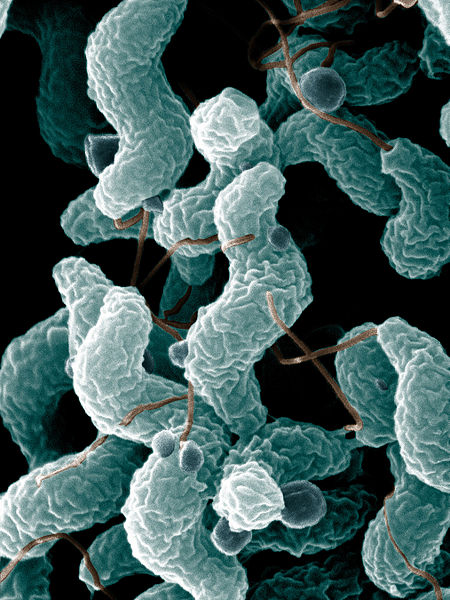
\includegraphics[width=6cm, trim=0 0 0 7.8]{Pictures/campy.jpg}
\end{minipage}
\end{frame}

\begin{frame}
\begin{center}
\simonbox{Goal 1: Determine the source of infection for human cases.}{mygreen}
\end{center}
\end{frame}

\begin{frame}{New Zealand campylobacteriosis cases}
\includegraphics[width=1.1\textwidth, trim=60 0 0 40]{Pictures/nz_Cases.pdf}
\end{frame}

\begin{frame}
\begin{center}
\simonbox{Goal 2: Does the proportion of human cases attributed to each source change seasonally?}{mygreen}
\end{center}
\end{frame}

\begin{frame}
\begin{center}
\simonbox{Goal 3: Is the intervention in the poultry industry the related to the drop in the number of cases after 2007?}{mygreen}
\end{center}
\end{frame}

\begin{frame}{Data from the Manawatu}
\begin{itemize}
\item Human isolates were collected from cases within the MidCentral DHB from 2005-2012.
\gap
\item During 2005-2008, isolates were collected from chicken, beef and lamb from supermarkets in the Manawatu.
\gap
\item In addition, water and environmental samples were collected from common swimming spots and neighbouring farms around the Manawatu.
\end{itemize}
\begin{center}
\begin{tabular}{ccccc}
Humans & Poultry & Sheep & Cattle & Water/Env\\
\hline
978 & 556 & 117 & 169 & 127\\
\end{tabular}
\end{center}
\end{frame}

\begin{frame}{How can we determine the origin of a human case?}
\begin{itemize}
\item The majority of cases are sporadic rather than being part of outbreaks.
\gap
\item Epidemiological information associated with a case may be minimal.
\gap
\item We often have no information on the exposure for sporadic cases.
\gap
\item Often the only thing we have is genotype information for each case.
\end{itemize}
\end{frame}

\begin{frame}{MLST for \emph{Campylobacter}}
\begin{minipage}{0.7\linewidth}
Seven housekeeping genes (loci).

\gap
Unique genes are assigned different numbers (alleles).

\gap
The combination of alleles at the seven loci gives the \textbf{multilocus sequence type}.
\end{minipage}
\begin{minipage}{0.25\linewidth}
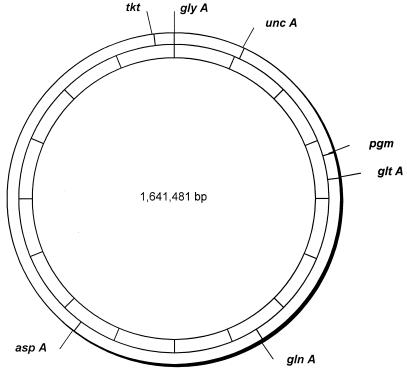
\includegraphics[width=4cm]{Pictures/campy_genome.jpg}
\end{minipage}
\begin{center}
\begin{tabular}{cccccccc}
ST & aspA & glnA & gltA & glyA & pgm & tkt & uncA\\
\hline
474 & 2 & 4 & 1 & 2 & 2 & 1 & 5\\
61 & 1 &      4 &      2 &      2 &      6 &       3     &  17\\
190   &  2    &   1     &  5   &    3   &    2    &   3    &   5\\
2381  &  175   &  251   &  216   &  282 &    359  &   293 &  102\\
48 & 2 & 4 & 1 & 2 & 7 & 1 & 5
\end{tabular}
\end{center}
\end{frame}

\begin{frame}{Human MLST types}
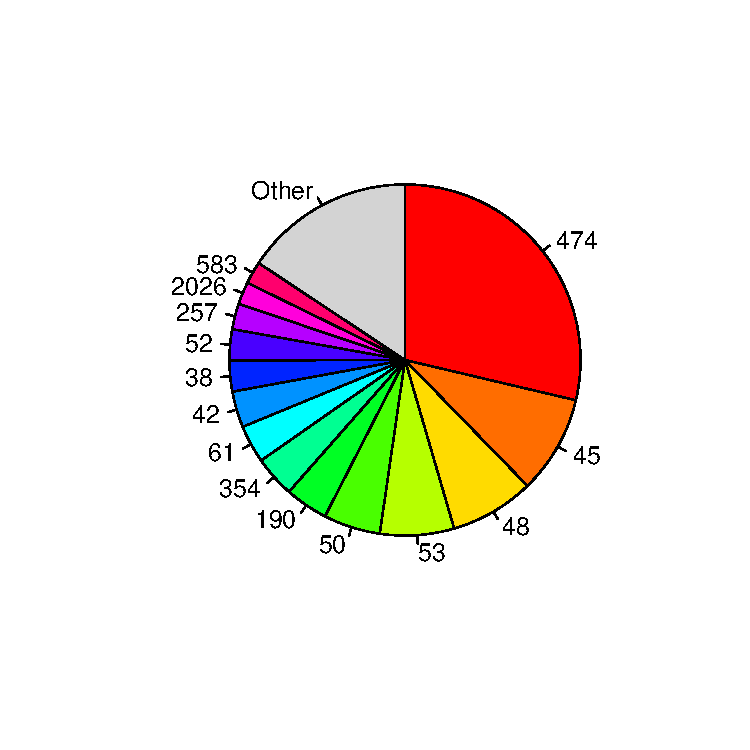
\includegraphics[width=0.9\textwidth, trim=50 70 50 70]{Pictures/humans.pdf}
\end{frame}

\begin{frame}{Source specific types}
\begin{center}
\begin{tabular}{cp{2cm}c}
\textbf{ST-474}: $n=60$ & & \textbf{ST-61}: $n=3$3\\
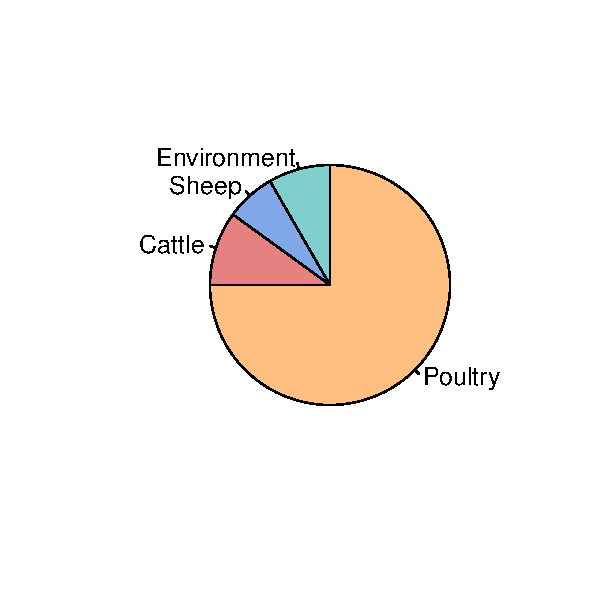
\includegraphics[width=0.25\textwidth,trim=80 60 80 60]{Pictures/474.pdf}
& &
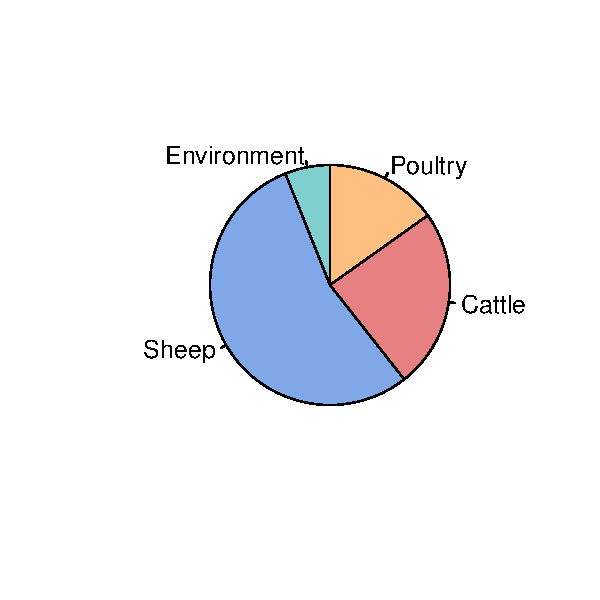
\includegraphics[width=0.25\textwidth,trim=80 60 80 60]{Pictures/61.pdf}\\
\textbf{ST-190}: $n=28$ & & \textbf{ST-2381}: $n=22$\\
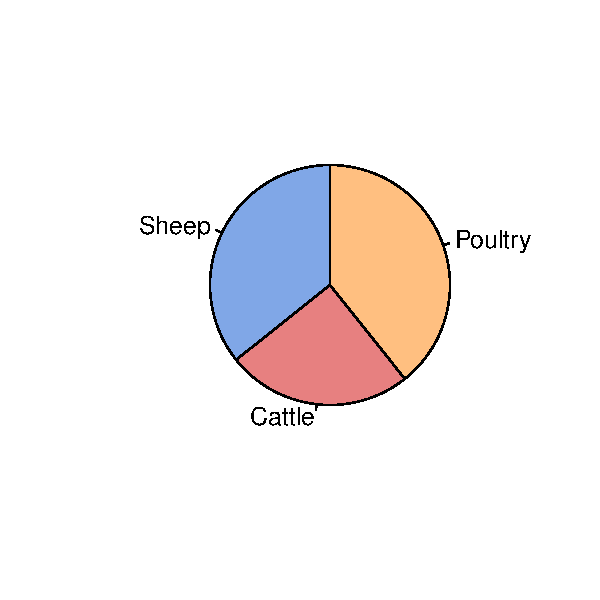
\includegraphics[width=0.25\textwidth,trim=80 40 80 60]{Pictures/190.pdf}
& &
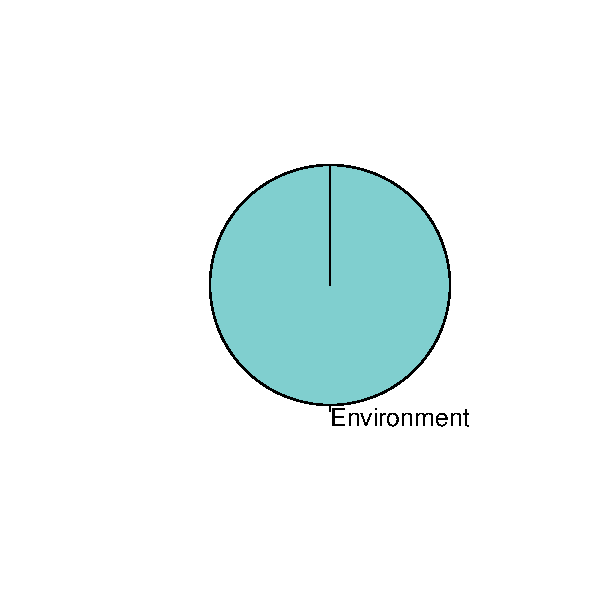
\includegraphics[width=0.25\textwidth,trim=80 40 80 60]{Pictures/2381.pdf}\\\end{tabular}
\end{center}
\end{frame}

\begin{frame}{Attribution using MLST}
Assign each human ST to the most likely source, given the distribution of STs on the source.

Use {\bf Bayes' Theorem}
\[
P(\mathsf{source}=k | \mathsf{ST}=i) = \frac{P(\mathsf{ST}=i|\mathsf{source}=k)P(\mathsf{source}=k)}{\sum_k P(\mathsf{ST}=i|\mathsf{source}=k)P(\mathsf{source}=k)}
\]
where
\begin{itemize}
\item $P(\mathsf{ST}=i|\mathsf{source}=k)$ is the distribution of STs on each source.
\gap
\item $P(\mathsf{source}=k)$ is the prior probability that an isolate picked at random is from source $k$.
\end{itemize}
\end{frame}

\begin{frame}{Island model {\small(D. Wilson, 2008)}}
Model the distribution of allelic profiles $P(\mathsf{ST}|\mathsf{source})$ on each source by assuming that the observed sequences arise due to:
\begin{itemize}
\item \textbf{Mutation}, where an allele at a locus is novel.
\gap
\item \textbf{Migration} between sources, where the allelic profile has been observed before in one of the sources, including the current one.
\gap
\item \textbf{Recombination}, where the allele at a given loci has been observed before but not in this allelic profile.
\end{itemize}
\end{frame}

\begin{frame}{Island model}
\begin{center}
\begin{tabular}{cccccccc}
ST & aspA & glnA & gltA & glyA & \hb{pgm} & tkt & uncA\\
474 & 2 & 4 & 1 & 2 & \hb{2} & 1 & 5\\
\hl{?} & \hl{2} & \hl{4} & \hl{1} & \hl{2} & \hb{29} & \hl{1} & \hl{5}\\
\end{tabular}
\end{center}

We have a novel allele at the pgm locus.  We assume this genotype has arisen through \textbf{mutation}.
\end{frame}

\begin{frame}{Island model}
\begin{center}
\begin{tabular}{cccccccc}
ST & aspA & glnA & gltA & glyA & \hb{pgm} & tkt & uncA\\
474 & 2 & 4 & 1 & 2 & \hb{2} & 1 & 5\\
\hl{?} & \hl{2} & \hl{4} & \hl{1} & \hl{2} & \hb{1} & \hl{1} & \hl{5}\\
\end{tabular}
\end{center}

The pgm allele looks familiar...

\begin{center}
\begin{tabular}{cccccccc}
ST & aspA & glnA & gltA & glyA & \hb{pgm} & tkt & uncA\\
45 & 4 & 7 & 10 & 4 & \hb{1} & 7 & 1\\
3718 & 2 & 4 & 1 & 4 & \hb{1} & 1 & 5\\
\end{tabular}
\end{center}

But we haven't seen this genotype before. We assume it arose through \textbf{recombination}.
\end{frame}

\begin{frame}{Island model}
\begin{center}
\begin{tabular}{cccccccc}
ST & aspA & glnA & gltA & glyA & \hb{pgm} & tkt & uncA\\
474 & 2 & 4 & 1 & 2 & \hb{2} & 1 & 5\\
\hl{?} & \hl{2} & \hl{4} & \hl{1} & \hl{2} & \hb{2} & \hl{1} & \hl{5}\\
\end{tabular}
\end{center}

This is just 474 - we've seen this before, but possibly not in this source. We assume it arose through \textbf{migration}.
\end{frame}

\begin{frame}{Island model}
The probability of observing $y=(y^1,y^2,\ldots,y^7)$ in source $k$ is
{\footnotesize
\[
\phi(y|k,X) = \sum_{c\in X} \frac{M_{S_ck}}{N_{S_c}} \prod_{l=1}^7 \left\{\begin{array}{ll}
\mu_k & \textsf{if $y^{l}$ is novel,}
\vspace{10pt}\\
(1-\mu_k)R_k\sum_{j=1}^K M_{jk}f^l_{y^lj} & \textsf{if $y^{l}\neq c^l$}
\vspace{10pt}\\
(1-\mu_k)\left[1 - R_k(1 - \sum_{j=1}^K M_{jk}f^l_{y^lj})\right] & \textsf{if $y^{l}=c^l$}
\end{array} \right.
\]}\\
where\vspace{-15pt}
{\small
\begin{itemize}
\item $X$ are the previously observed sequences.
\item $c$ comes from source $S_c$.
\item $\mu_k$ be the probability of a novel mutant allele.
\item $R_k$ be the probability that a type has undergone recombination.
\item $M_{jk}$ be the probability of an allele migrating from source $j$ to $k$.
\item $f^l_{aj}$ be the frequency with which allele $a$ has been observed at locus $l$ in those genotypes sampled from source $j$.
\end{itemize}
}
\end{frame}

\begin{frame}{Estimating parameters}
The likelihood for observing source types $Y$ given $\mu$, $M$, and $R$ may be approximated using a leave-one-out approach.
\[
p(Y|\mu,M,R) \sim \prod_{y \in Y} \phi(y|S_y, Y - \{y\}).
\]
We fit this using MCMC with switching and lognormal Metropolis-Hastings proposals for $\mu$, $M$, and $R$.
\end{frame}

\begin{frame}{Attribution of human isolates to sources}
Let $F_{k}$ be the proportion of human isolates attributed to source $k$.

Then the posterior distribution for $F_k$ given human isolates $H$ and source isolates $Y$ is
\[
p(F_k| H, Y) \propto \prod_{h\in H} \sum_k F_k\phi(h|k,Y) p(F_k)
\]
where $p(F_k)$ is the prior where we assume each source is equally likely.

This depends on $\mu$, $M$ and $R$, thus for each posterior sample from their MCMC chain we run a side chain to estimate $F_k$.
\end{frame}

\begin{frame}{Proportion of human cases attributed to each source}
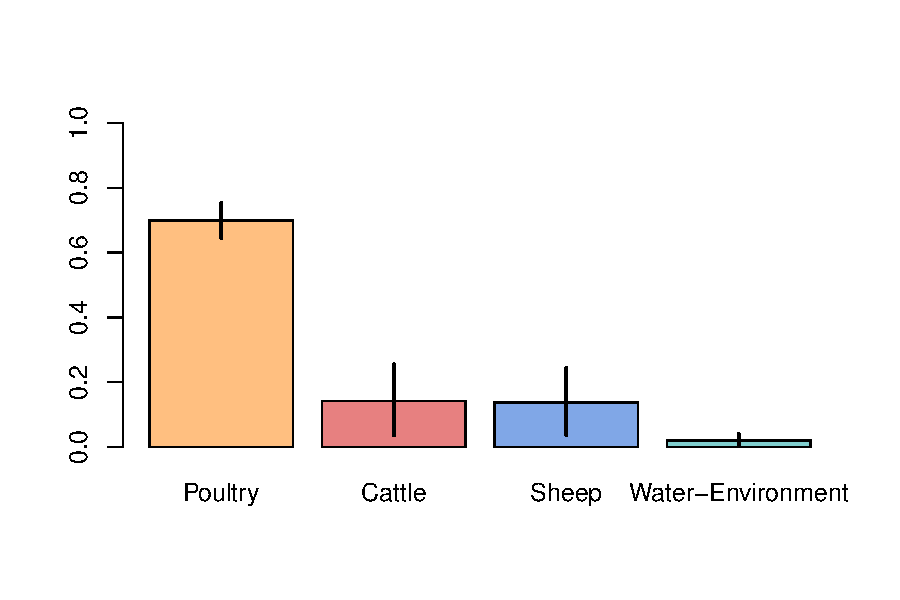
\includegraphics[width=\textwidth, trim=40 0 40 0]{Pictures/island/overall_prop.pdf}
\end{frame}

\begin{frame}{Migration, mutation, and recombination}
\hspace{-30pt}
\begin{minipage}{0.5\linewidth}
\begin{tabular}{cc}
Poultry & Cattle\\
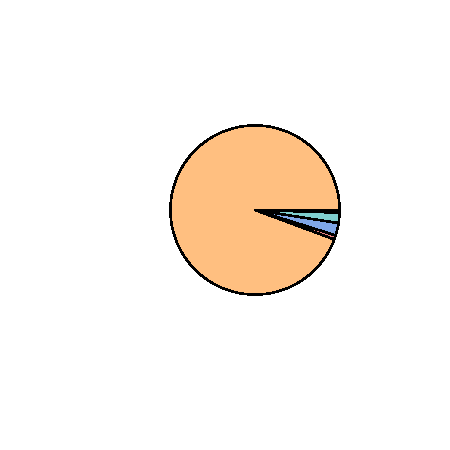
\includegraphics[width=1.5in, trim=70 60 40 60]{Pictures/island/migration_mutation1.pdf}
& 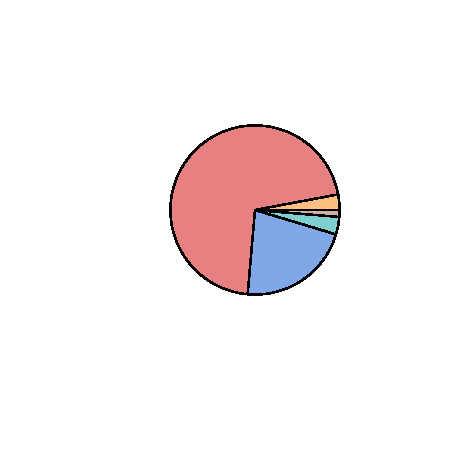
\includegraphics[width=1.5in, trim=70 60 40 60]{Pictures/island/migration_mutation2.pdf}\\
Sheep & Water-Environment\\
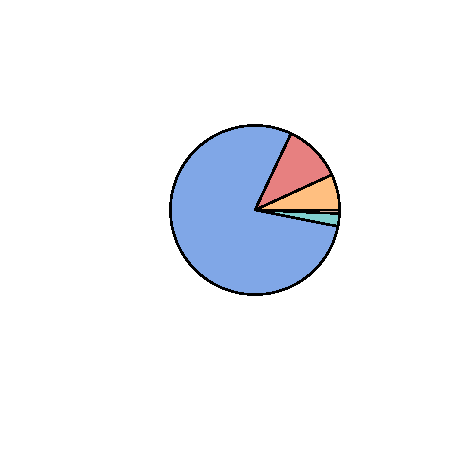
\includegraphics[width=1.5in, trim=70 60 40 60]{Pictures/island/migration_mutation3.pdf}
&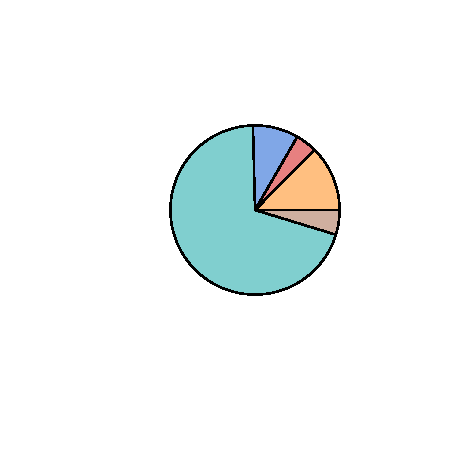
\includegraphics[width=1.5in, trim=70 60 40 60]{Pictures/island/migration_mutation4.pdf}
\end{tabular}
\end{minipage}
\hspace{110pt}
\begin{minipage}{0.2\linewidth}
Recombination
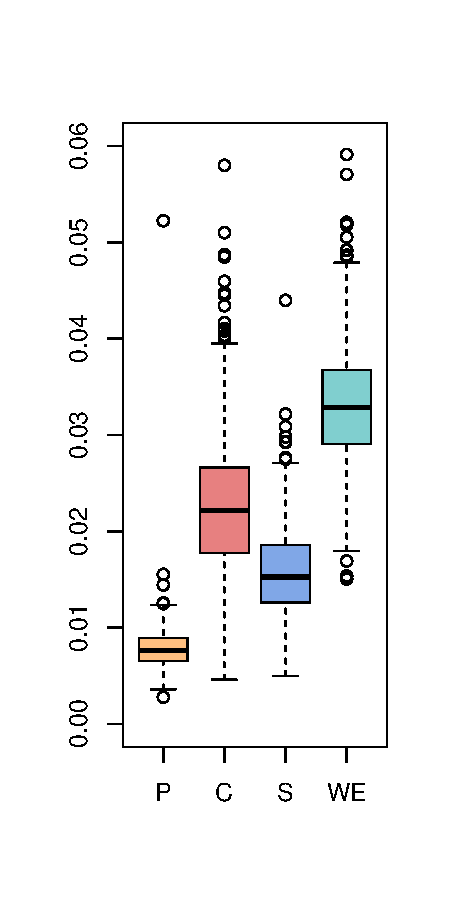
\includegraphics[width=1.8in, trim=70 30 -70 40]{Pictures/island/recombination.pdf}
\end{minipage}
%\end{center}
\end{frame}

\begin{frame}{Seasonal model for $F_k$}
Suppose $F_k$ can change through time, and let
\[
F_{kt} = \left\{\begin{array}{ll}\displaystyle\frac{e^{-f_{kt}}}{1 + \sum_{k=1}^{K-1} e^{-f_{kt}}} & k=1\ldots K-1,
\vspace{10pt}\\
\displaystyle\frac{1}{1 + \sum_{k=1}^{K-1} e^{-f_{kt}}}& k=K.\end{array}\right.
\]
where
\begin{align*}
f_{kt} &= \sum_{i=1}^4 \alpha_{ik} {\bf 1}_{t \in \mathsf{Season}_i} + \beta_k {\bf 1}_{t \geq 2007} +\epsilon_{kt},\\
\epsilon_{kt} & \sim \mathsf{Normal}(\rho_k \epsilon_{k(t-1)}, \sigma^2_{k}).
\end{align*}
\vspace{-30pt}
\end{frame}

\begin{frame}{Proportions: pre-2007}
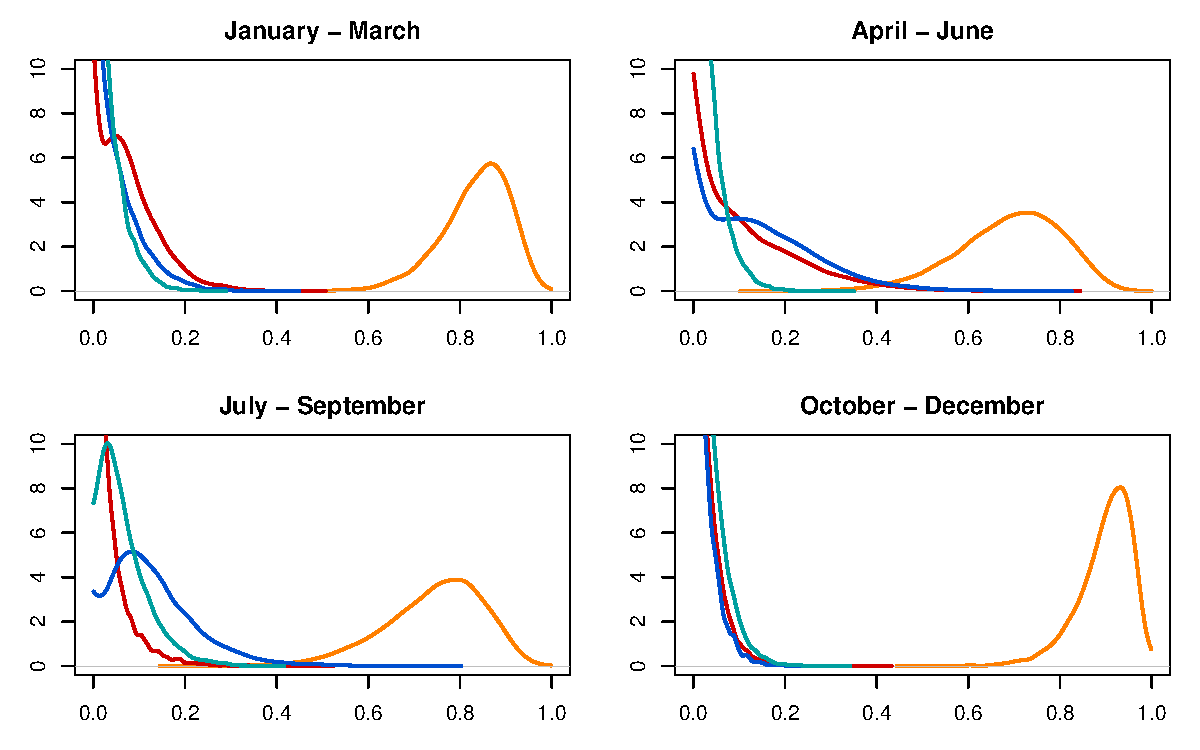
\includegraphics[width=\textwidth, trim=40 0 40 0]{Pictures/island/seasonal_props1.pdf}
\end{frame}

\begin{frame}{Proportions: post-2007}
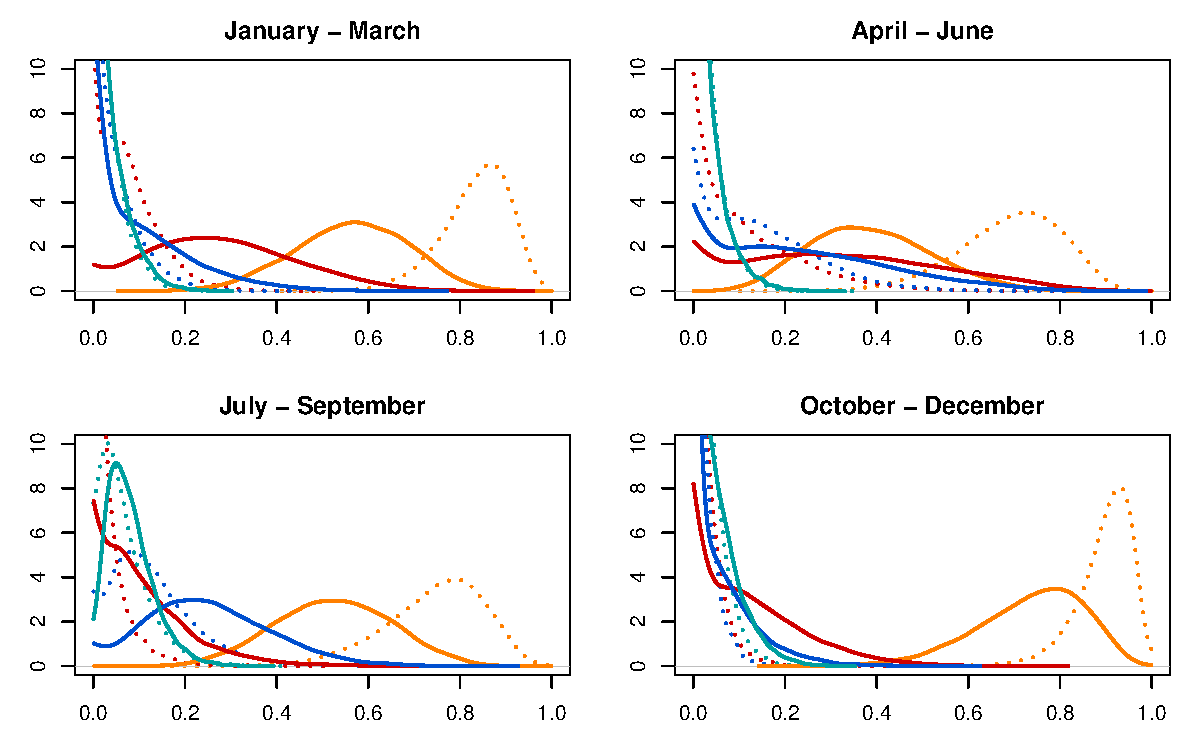
\includegraphics[width=\textwidth, trim=40 0 40 0]{Pictures/island/seasonal_props2.pdf}
\end{frame}

\begin{frame}{Totals: pre-2007}
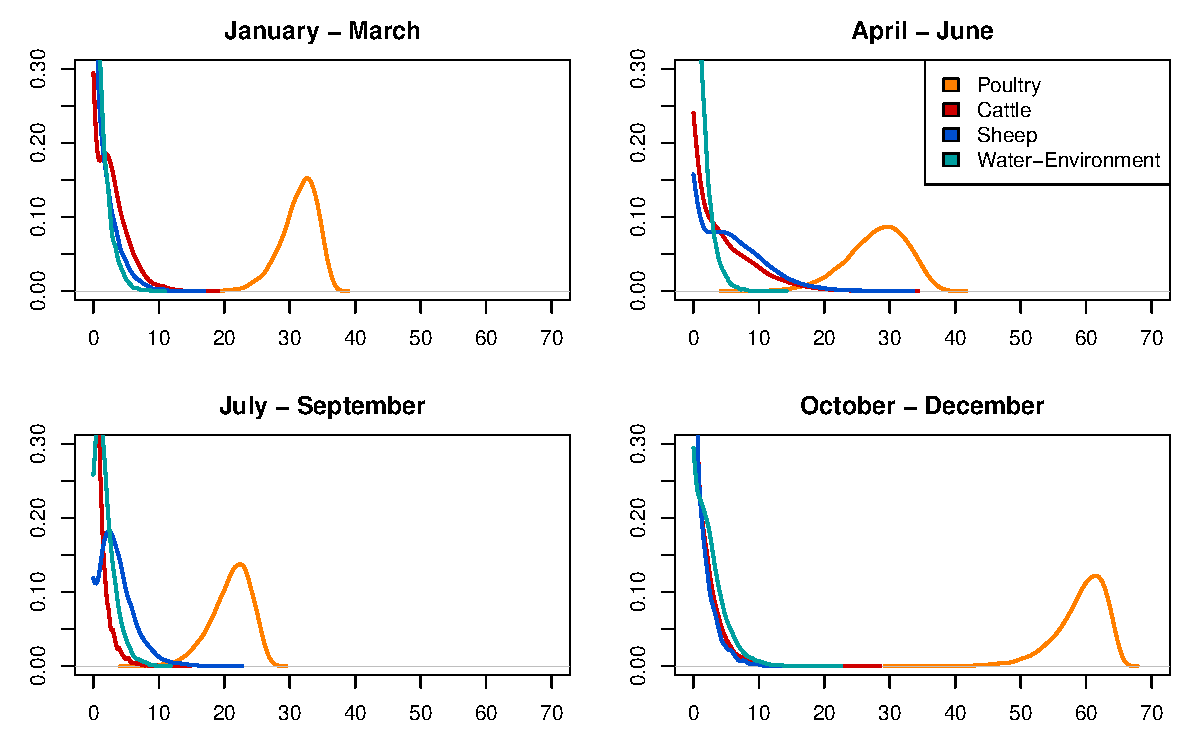
\includegraphics[width=\textwidth, trim=40 0 40 0]{Pictures/island/seasonal_totals1.pdf}
\end{frame}

\begin{frame}{Totals: post-2007}
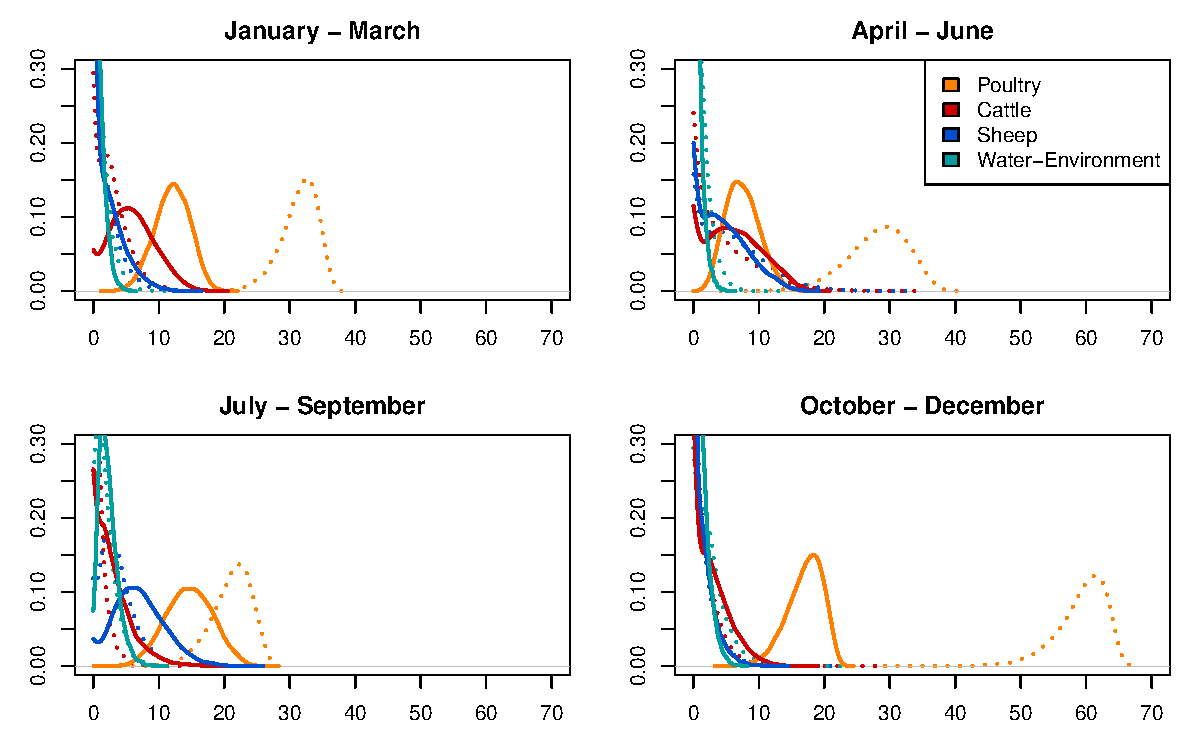
\includegraphics[width=\textwidth, trim=40 0 40 0]{Pictures/island/seasonal_totals2.pdf}
\end{frame}

\begin{frame}{\emph{Campylobacter} in the Manawatu}
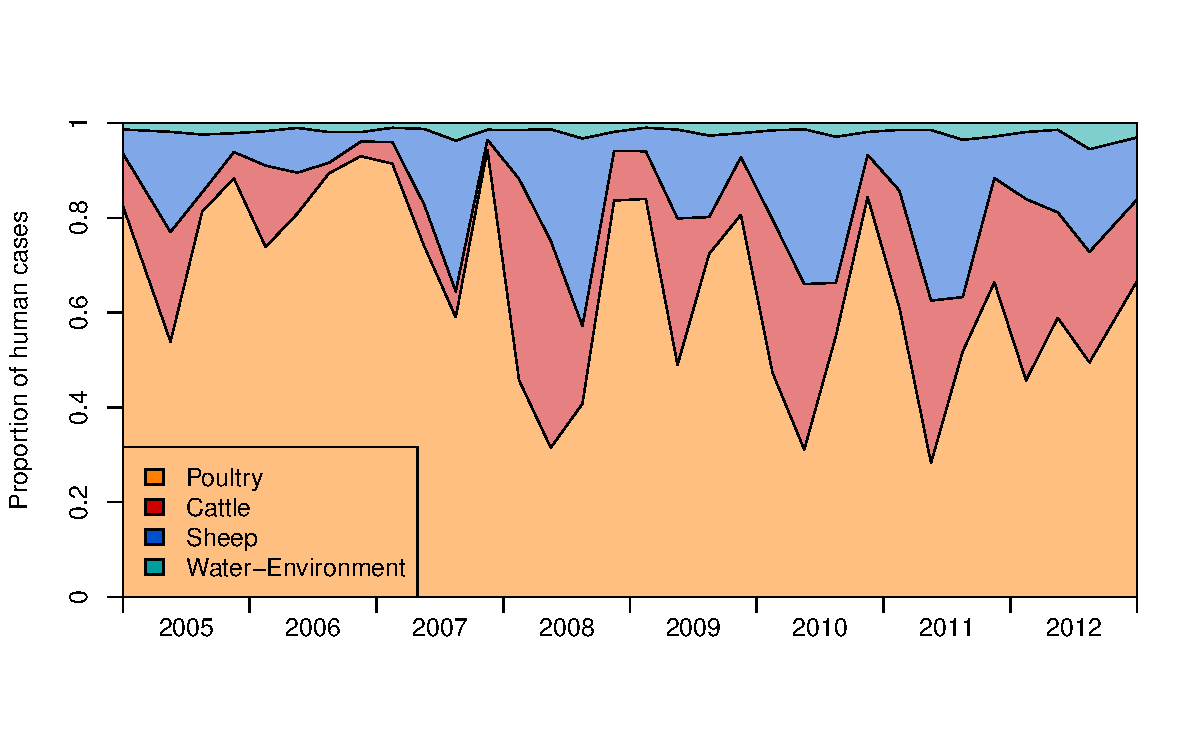
\includegraphics[width=\textwidth, trim=40 0 40 0]{Pictures/island/proportions.pdf}
\end{frame}

\begin{frame}{\emph{Campylobacter} in the Manawatu}
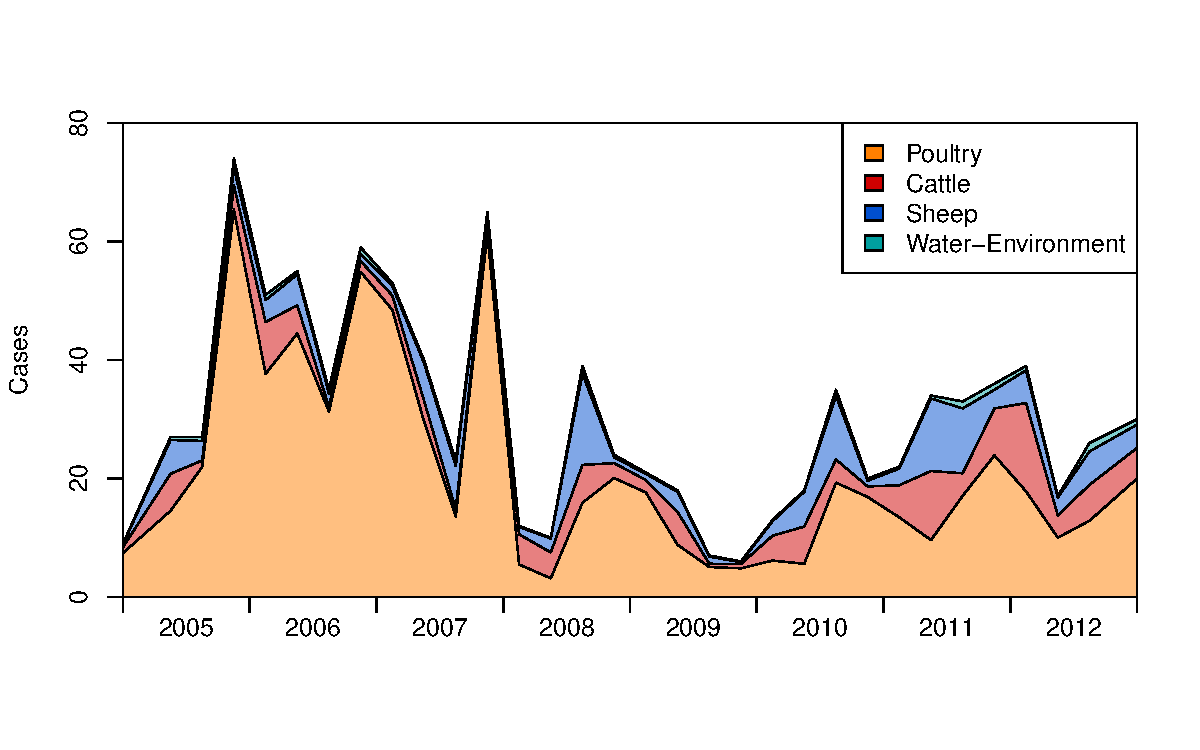
\includegraphics[width=\textwidth, trim=40 0 40 0]{Pictures/island/totals.pdf}
\end{frame}

\begin{frame}{Summary}
\begin{itemize}
\item Genotyping information allows us to assign human cases to their most likely source.
\gap
\item The majority of cases are attributed to poultry.
\gap
\item There are interesting seasonal trends, with more poultry cases in summer and more ruminant cases in winter.
\gap
\item The water/environmental strains don't seem to be associated with human illness, but do show higher probabilities of mutation and recombination.
\gap
\item The poultry intervention in 2007 appears to be the main reason for the decrease in total human cases.
\end{itemize}
\end{frame}

%\begin{frame}{Source means and correlation}
%\includegraphics[width=\textwidth]{Pictures/island/mean_correlation.pdf}
%\end{frame}

\begin{frame}{Thanks for listening}
\begin{center}
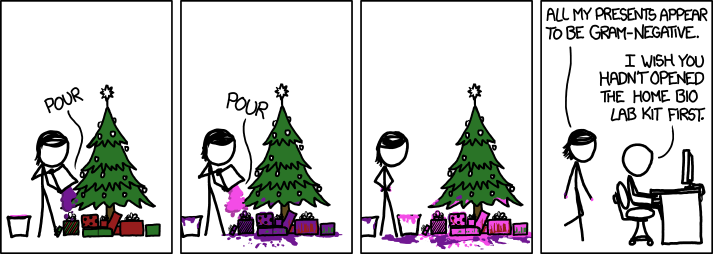
\includegraphics[width=3.5in]{Pictures/questions}
\end{center}
\end{frame}

\begin{frame}{\emph{Campylobacter} in the Manawatu}
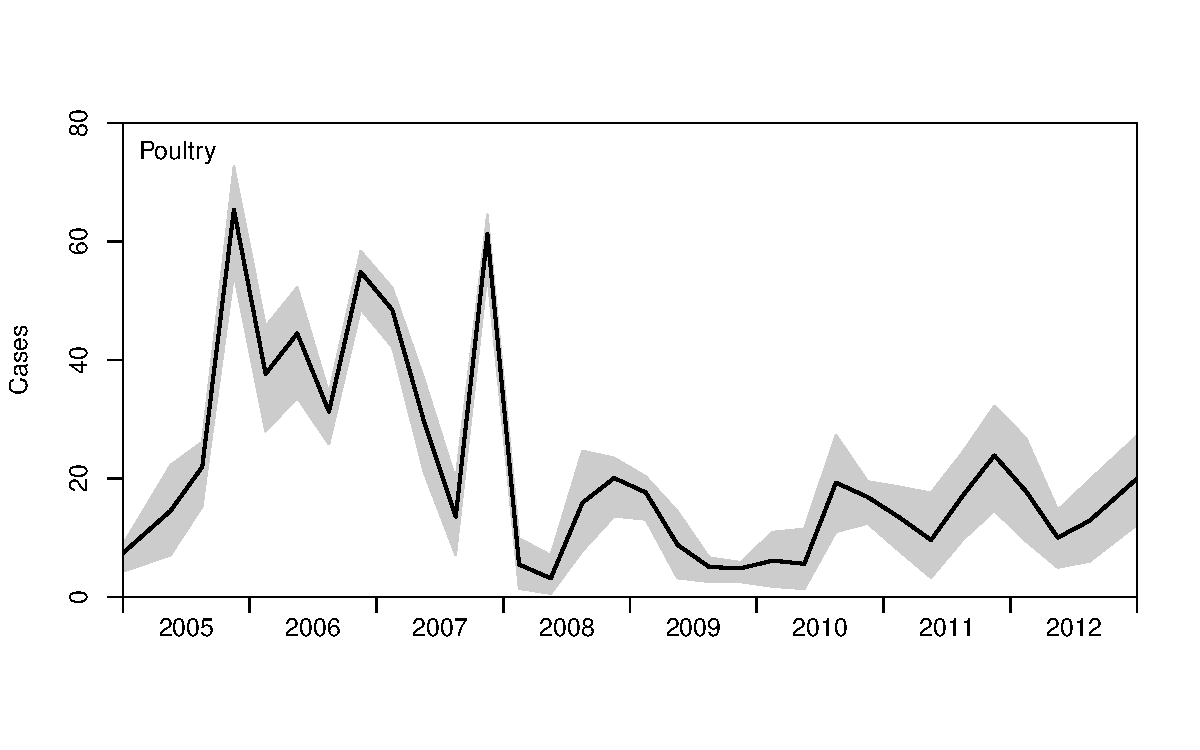
\includegraphics[width=\textwidth, trim=40 0 40 0]{Pictures/island/totals_Poultry.pdf}
\end{frame}

\begin{frame}{\emph{Campylobacter} in the Manawatu}
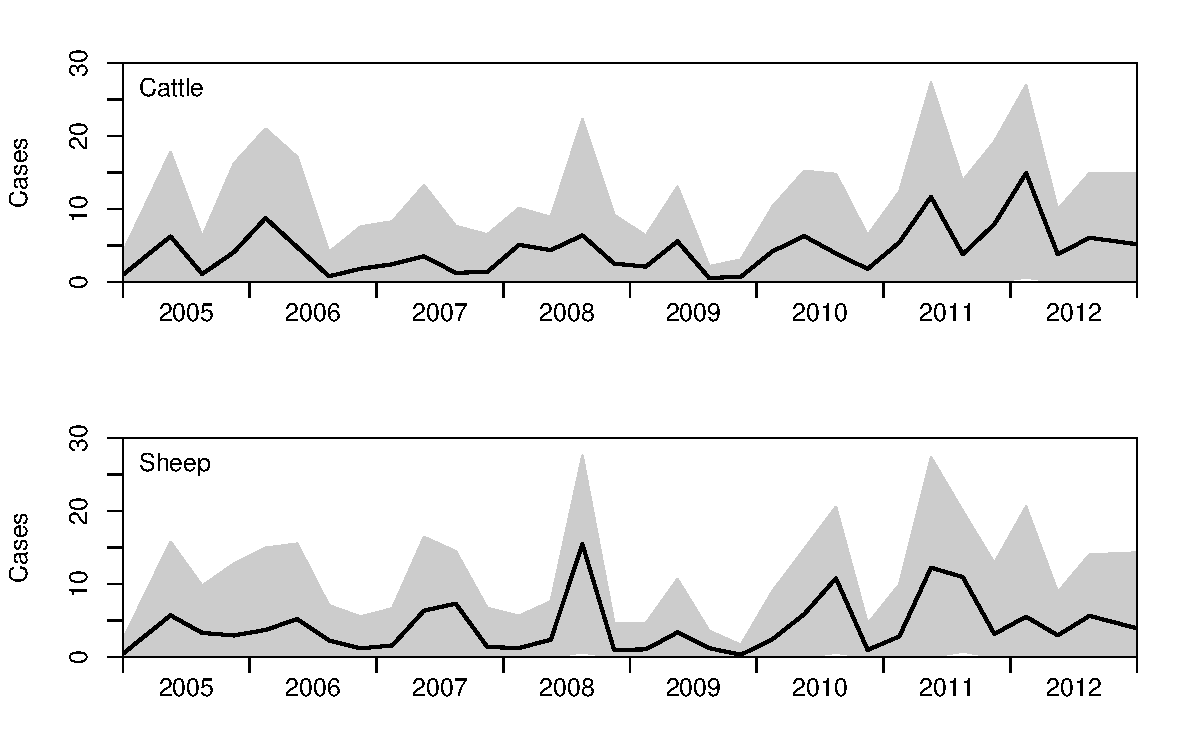
\includegraphics[width=\textwidth, trim=40 0 40 0]{Pictures/island/totals_ruminants_combined.pdf}
\end{frame}

\begin{frame}{\emph{Campylobacter} in the Manawatu}
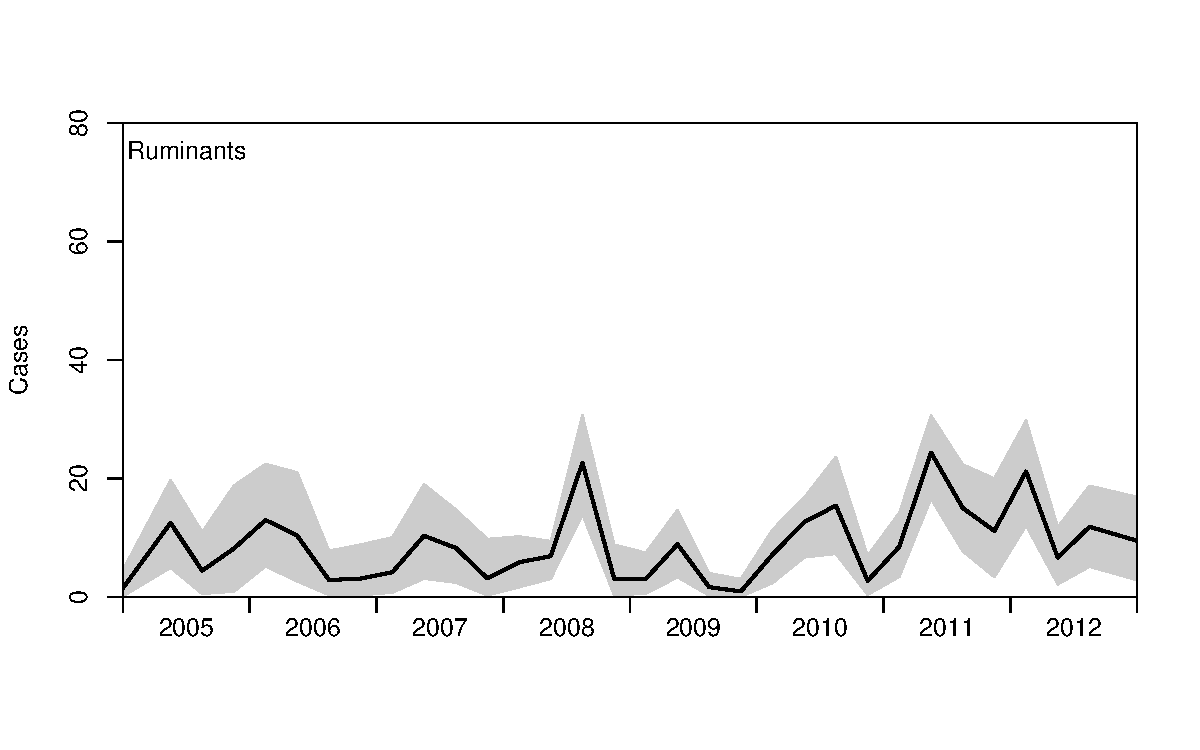
\includegraphics[width=\textwidth, trim=40 0 40 0]{Pictures/island/ruminants/totals_Ruminants.pdf}
\end{frame}

\begin{frame}{\emph{Campylobacter} in the Manawatu}
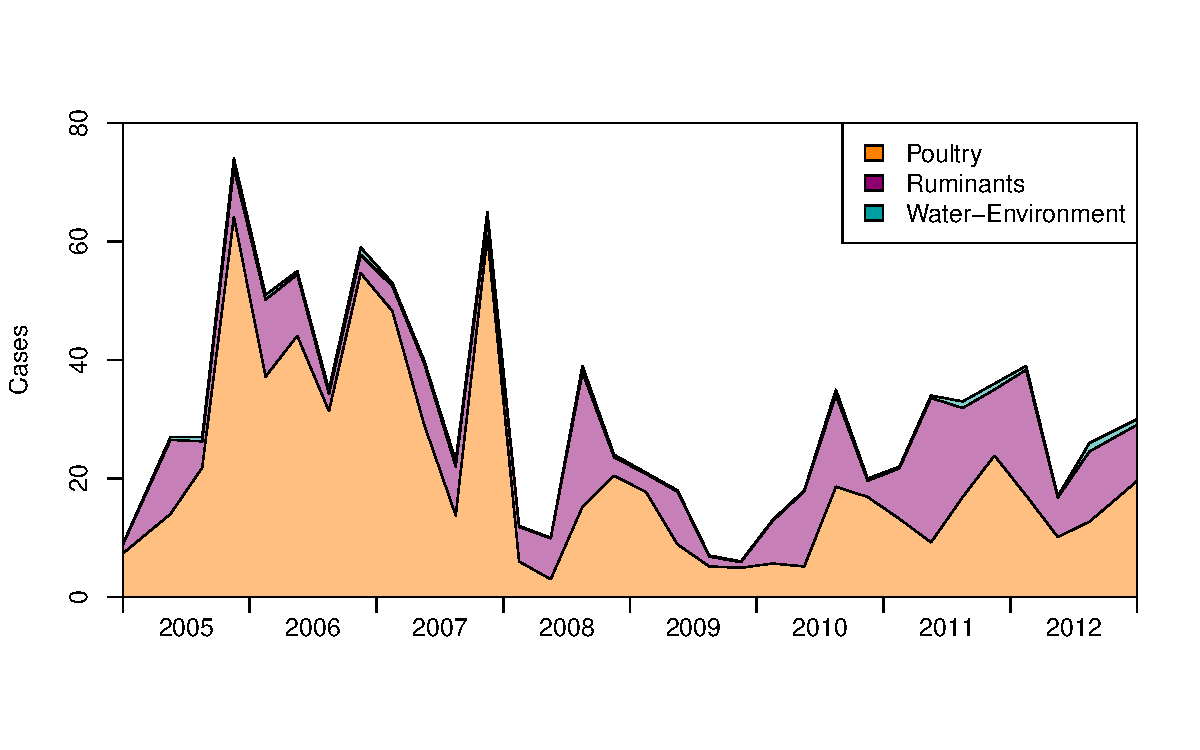
\includegraphics[width=\textwidth, trim=40 0 40 0]{Pictures/island/ruminants/totals.pdf}
\end{frame}

\begin{frame}{\emph{Campylobacter} in the Manawatu}
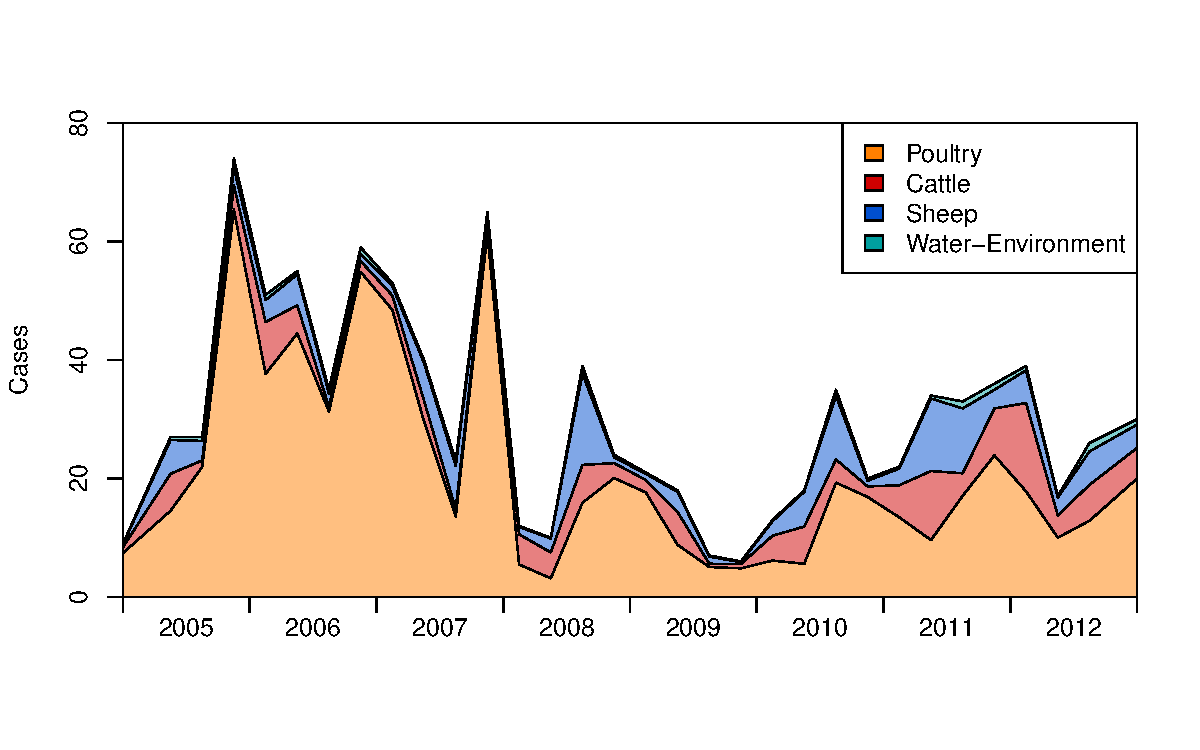
\includegraphics[width=\textwidth, trim=40 0 40 0]{Pictures/island/totals.pdf}
\end{frame}

\end{document}
